\documentclass{article}\usepackage[]{graphicx}\usepackage[]{color}
%% maxwidth is the original width if it is less than linewidth
%% otherwise use linewidth (to make sure the graphics do not exceed the margin)
\makeatletter
\def\maxwidth{ %
  \ifdim\Gin@nat@width>\linewidth
    \linewidth
  \else
    \Gin@nat@width
  \fi
}
\makeatother

\definecolor{fgcolor}{rgb}{0.345, 0.345, 0.345}
\newcommand{\hlnum}[1]{\textcolor[rgb]{0.686,0.059,0.569}{#1}}%
\newcommand{\hlstr}[1]{\textcolor[rgb]{0.192,0.494,0.8}{#1}}%
\newcommand{\hlcom}[1]{\textcolor[rgb]{0.678,0.584,0.686}{\textit{#1}}}%
\newcommand{\hlopt}[1]{\textcolor[rgb]{0,0,0}{#1}}%
\newcommand{\hlstd}[1]{\textcolor[rgb]{0.345,0.345,0.345}{#1}}%
\newcommand{\hlkwa}[1]{\textcolor[rgb]{0.161,0.373,0.58}{\textbf{#1}}}%
\newcommand{\hlkwb}[1]{\textcolor[rgb]{0.69,0.353,0.396}{#1}}%
\newcommand{\hlkwc}[1]{\textcolor[rgb]{0.333,0.667,0.333}{#1}}%
\newcommand{\hlkwd}[1]{\textcolor[rgb]{0.737,0.353,0.396}{\textbf{#1}}}%
\let\hlipl\hlkwb

\usepackage{framed}
\makeatletter
\newenvironment{kframe}{%
 \def\at@end@of@kframe{}%
 \ifinner\ifhmode%
  \def\at@end@of@kframe{\end{minipage}}%
  \begin{minipage}{\columnwidth}%
 \fi\fi%
 \def\FrameCommand##1{\hskip\@totalleftmargin \hskip-\fboxsep
 \colorbox{shadecolor}{##1}\hskip-\fboxsep
     % There is no \\@totalrightmargin, so:
     \hskip-\linewidth \hskip-\@totalleftmargin \hskip\columnwidth}%
 \MakeFramed {\advance\hsize-\width
   \@totalleftmargin\z@ \linewidth\hsize
   \@setminipage}}%
 {\par\unskip\endMakeFramed%
 \at@end@of@kframe}
\makeatother

\definecolor{shadecolor}{rgb}{.97, .97, .97}
\definecolor{messagecolor}{rgb}{0, 0, 0}
\definecolor{warningcolor}{rgb}{1, 0, 1}
\definecolor{errorcolor}{rgb}{1, 0, 0}
\newenvironment{knitrout}{}{} % an empty environment to be redefined in TeX

\usepackage{alltt}

% \usepackage[utf8]{inputenc}
\usepackage{amsmath}
\usepackage{fancyhdr}
\usepackage{array}
\usepackage{longtable}
\usepackage{graphicx}
\usepackage{color}
\usepackage[letterpaper, margin=1in]{geometry}
\usepackage{lscape}
\newcommand{\blandscape}{\begin{landscape}}
\newcommand{\elandscape}{\end{landscape}}
\usepackage{dcolumn}
\usepackage{bbm}
\usepackage{threeparttable}
\usepackage{booktabs}
\usepackage{expex}
\usepackage{pdflscape}
\usepackage{rotating, graphicx}
\usepackage{tabulary}
\usepackage{lscape}
\usepackage{makecell}
\usepackage{algorithm}
\usepackage{multirow}
\usepackage{colortbl}
\usepackage{longtable}
\usepackage{array}
\usepackage{multirow}
\usepackage{wrapfig}
\usepackage{float}
\usepackage{pdflscape}
\usepackage{tabu}
\usepackage{threeparttable}

\title{%
Homework 3\\
\large Applied Mutlivariate Analysis}
\date{September 22, 2018}
\author{Emorie Beck}
\IfFileExists{upquote.sty}{\usepackage{upquote}}{}
\begin{document}
\maketitle
% \SweaveOpts{concordance=TRUE}

\section{Workspace}
\subsection{Packages}



\begin{knitrout}
\definecolor{shadecolor}{rgb}{0.969, 0.969, 0.969}\color{fgcolor}\begin{kframe}
\begin{alltt}
\hlkwd{library}\hlstd{(car)}
\hlkwd{library}\hlstd{(knitr)}
\hlkwd{library}\hlstd{(psych)}
\hlkwd{library}\hlstd{(lavaan)}
\hlkwd{library}\hlstd{(semPlot)}
\hlkwd{library}\hlstd{(kableExtra)}
\hlkwd{library}\hlstd{(multcomp)}
\hlkwd{library}\hlstd{(lme4)}
\hlkwd{library}\hlstd{(plyr)}
\hlkwd{library}\hlstd{(tidyverse)}
\hlkwd{library}\hlstd{(MVN)}
\end{alltt}
\end{kframe}
\end{knitrout}



\subsection{data}
The file, Set\_5.csv, contains data from a study in which college students completed the NEO-PI Personality Inventory. This 240-item scale purportedly measures the Big Five personality dimensions, assumed to be fairly independent. The inventory is scored on 6 subscales per dimension, listed below. The file contains the subscale scores, rather than the individual items, which should help reduce the impact of the small sample size.\\

Neuroticism: Anxiety\\
Neuroticism: Angry\_Hostility\\
Neuroticism: Depression\\
Neuroticism: Self\_Consciousness\\
Neuroticism: Impulsiveness\\
Neuroticism: Vulnerability\\
Extraversion: Warmth\\
Extraversion: Gregariousness\\
Extraversion: Assertiveness\\
Extraversion: Activity\\
Extraversion: Excitement\_Seeking\\
Extraversion: Positive\_Emotions\\
Openness: Fantasy\\
Openness: Aesthetics\\
Openness: Feelings\\
Openness: Actions\\
Openness: Ideas\\
Openness: Values\\
Agreeableness: Trust\\
Agreeableness: Straightforwardness \\
Agreeableness: Altruism\\
Agreeableness: Compliance\\
Agreeableness: Modesty\\
Agreeableness: Tender\_Mindedness\\
Conscientiousness: Competence\\
Conscientiousness: Order\\
Conscientiousness: Dutifulness\\
Conscientiousness: Achievement\_Striving \\
Conscientiousness: Self\_Discipline\\
Conscientiousness: Deliberation\\

\begin{knitrout}
\definecolor{shadecolor}{rgb}{0.969, 0.969, 0.969}\color{fgcolor}\begin{kframe}
\begin{alltt}
\hlstd{wd} \hlkwb{<-} \hlstr{"https://github.com/emoriebeck/homeworks/raw/master/multivariate/homeworks/homework6"}

\hlstd{dat} \hlkwb{<-} \hlkwd{sprintf}\hlstd{(}\hlstr{"%s/Set_5(1).csv"}\hlstd{, wd)} \hlopt
  \hlkwd{read.csv}\hlstd{(.,} \hlkwc{stringsAsFactors} \hlstd{= F)}

\hlkwd{head}\hlstd{(dat)}
\end{alltt}
\begin{verbatim}
##   ID Anxiety Angry_Hostility Depression Self_Consciousness Impulsiveness
## 1  2   2.625           2.000      1.750           2.250000         2.625
## 2  3   3.625           2.875      3.000           3.500000         4.250
## 3  4   3.000           2.750      2.625           2.875000         3.000
## 4  5   4.375           3.125      4.500           4.000000         3.875
## 5  6   3.500           2.875      3.000           2.571429         3.625
## 6  7   4.000           4.125      2.875           2.375000         4.000
##   Vulnerability   Warmth Gregariousness Assertiveness Activity
## 1      2.166667 4.666667          4.000      3.000000 4.833333
## 2      2.125000 4.500000          2.750      2.625000 3.000000
## 3      2.875000 3.750000          3.125      2.375000 3.250000
## 4      3.750000 3.250000          2.250      2.500000 1.875000
## 5      2.750000 3.750000          3.125      3.285714 3.500000
## 6      3.125000 3.500000          2.625      3.375000 3.125000
##   Excitement_Seeking Positive_Emotions  Fantasy Aesthetics Feelings
## 1              3.500             4.750 3.857143   3.571429 4.666667
## 2              2.875             3.500 3.500000   4.125000 3.625000
## 3              3.875             3.375 3.375000   3.500000 3.250000
## 4              2.750             2.625 3.000000   3.750000 4.250000
## 5              3.750             3.625 3.125000   1.625000 3.125000
## 6              2.000             3.375 3.500000   2.000000 3.250000
##    Actions Ideas Values Trust Straightforwardness Altruism Compliance
## 1 2.571429 4.400  4.600 5.000            2.166667 4.833333      2.750
## 2 3.000000 3.875  3.125 3.250            3.750000 3.625000      3.125
## 3 2.375000 4.125  3.500 3.250            3.125000 4.000000      3.750
## 4 3.375000 2.750  4.125 3.000            3.428571 3.875000      4.000
## 5 2.750000 2.500  3.625 3.375            3.250000 4.125000      3.625
## 6 2.625000 1.125  3.625 2.500            2.875000 3.000000      2.250
##   Modesty Tender_Mindedness Competence Order Dutifulness
## 1   4.000          3.833333       4.50 3.625    3.285714
## 2   2.625          3.250000       3.00 2.250    3.875000
## 3   2.750          3.250000       3.75 3.250    3.750000
## 4   4.125          3.750000       2.75 3.000    2.875000
## 5   3.375          3.375000       3.75 4.000    3.750000
## 6   2.625          3.375000       3.00 3.625    2.625000
##   Achievement_Striving Self_Discipline Deliberation
## 1             4.333333           4.250        2.875
## 2             2.750000           3.750        3.500
## 3             3.375000           3.375        3.125
## 4             2.875000           2.625        3.250
## 5             3.375000           2.875        3.375
## 6             3.000000           2.625        2.625
\end{verbatim}
\end{kframe}
\end{knitrout}

\begin{knitrout}
\definecolor{shadecolor}{rgb}{0.969, 0.969, 0.969}\color{fgcolor}\begin{kframe}
\begin{alltt}
\hlstd{source} \hlkwb{<-} \hlkwd{tribble}\hlstd{(}
\hlopt{~}\hlstd{Factor,} \hlopt{~}\hlstd{Facet,}
\hlstr{"Neuroticism"}\hlstd{,} \hlstr{"Anxiety"}\hlstd{,}
\hlstr{"Neuroticism"}\hlstd{,} \hlstr{"Angry_Hostility"}\hlstd{,}
\hlstr{"Neuroticism"}\hlstd{,} \hlstr{"Depression"}\hlstd{,}
\hlstr{"Neuroticism"}\hlstd{,} \hlstr{"Self_Consciousness"}\hlstd{,}
\hlstr{"Neuroticism"}\hlstd{,} \hlstr{"Impulsiveness"}\hlstd{,}
\hlstr{"Neuroticism"}\hlstd{,} \hlstr{"Vulnerability"}\hlstd{,}
\hlstr{"Extraversion"}\hlstd{,} \hlstr{"Warmth"}\hlstd{,}
\hlstr{"Extraversion"}\hlstd{,} \hlstr{"Gregariousness"}\hlstd{,}
\hlstr{"Extraversion"}\hlstd{,} \hlstr{"Assertiveness"}\hlstd{,}
\hlstr{"Extraversion"}\hlstd{,} \hlstr{"Activity"}\hlstd{,}
\hlstr{"Extraversion"}\hlstd{,} \hlstr{"Excitement_Seeking"}\hlstd{,}
\hlstr{"Extraversion"}\hlstd{,} \hlstr{"Positive_Emotions"}\hlstd{,}
\hlstr{"Openness"}\hlstd{,} \hlstr{"Fantasy"}\hlstd{,}
\hlstr{"Openness"}\hlstd{,} \hlstr{"Aesthetics"}\hlstd{,}
\hlstr{"Openness"}\hlstd{,} \hlstr{"Feelings"}\hlstd{,}
\hlstr{"Openness"}\hlstd{,} \hlstr{"Actions"}\hlstd{,}
\hlstr{"Openness"}\hlstd{,} \hlstr{"Ideas"}\hlstd{,}
\hlstr{"Openness"}\hlstd{,} \hlstr{"Values"}\hlstd{,}
\hlstr{"Agreeableness"}\hlstd{,} \hlstr{"Trust"}\hlstd{,}
\hlstr{"Agreeableness"}\hlstd{,} \hlstr{"Straightforwardness"} \hlstd{,}
\hlstr{"Agreeableness"}\hlstd{,} \hlstr{"Altruism"}\hlstd{,}
\hlstr{"Agreeableness"}\hlstd{,} \hlstr{"Compliance"}\hlstd{,}
\hlstr{"Agreeableness"}\hlstd{,} \hlstr{"Modesty"}\hlstd{,}
\hlstr{"Agreeableness"}\hlstd{,} \hlstr{"Tender_Mindedness"}\hlstd{,}
\hlstr{"Conscientiousness"}\hlstd{,} \hlstr{"Competence"}\hlstd{,}
\hlstr{"Conscientiousness"}\hlstd{,} \hlstr{"Order"}\hlstd{,}
\hlstr{"Conscientiousness"}\hlstd{,} \hlstr{"Dutifulness"}\hlstd{,}
\hlstr{"Conscientiousness"}\hlstd{,} \hlstr{"Achievement_Striving"}\hlstd{,}
\hlstr{"Conscientiousness"}\hlstd{,} \hlstr{"Self_Discipline"}\hlstd{,}
\hlstr{"Conscientiousness"}\hlstd{,} \hlstr{"Deliberation"}
\hlstd{)}

\hlstd{dat} \hlkwb{<-} \hlstd{dat} \hlopt \hlkwd{select}\hlstd{(ID, source}\hlopt{$}\hlstd{Facet)}
\end{alltt}
\end{kframe}
\end{knitrout}

\subsection{Check for Outliers}
\begin{knitrout}
\definecolor{shadecolor}{rgb}{0.969, 0.969, 0.969}\color{fgcolor}\begin{kframe}
\begin{alltt}
\hlstd{dat2} \hlkwb{<-} \hlstd{dat} \hlopt \hlkwd{select}\hlstd{(}\hlopt{-}\hlstd{ID, )} \hlopt \hlstd{data.frame}
\hlkwd{rownames}\hlstd{(dat2)} \hlkwb{<-} \hlstd{dat}\hlopt{$}\hlstd{ID} \hlcom{#1:nrow(dat2)}
\hlstd{(mv} \hlkwb{<-} \hlkwd{mvn}\hlstd{(dat2,}\hlkwc{mvnTest}\hlstd{=}\hlstr{"mardia"}\hlstd{,} \hlkwc{multivariatePlot}\hlstd{=}\hlstr{"qq"}\hlstd{,}\hlkwc{multivariateOutlierMethod}\hlstd{=}\hlstr{"quan"}\hlstd{,}\hlkwc{showOutliers}\hlstd{=}\hlnum{TRUE}\hlstd{))}
\end{alltt}
\end{kframe}
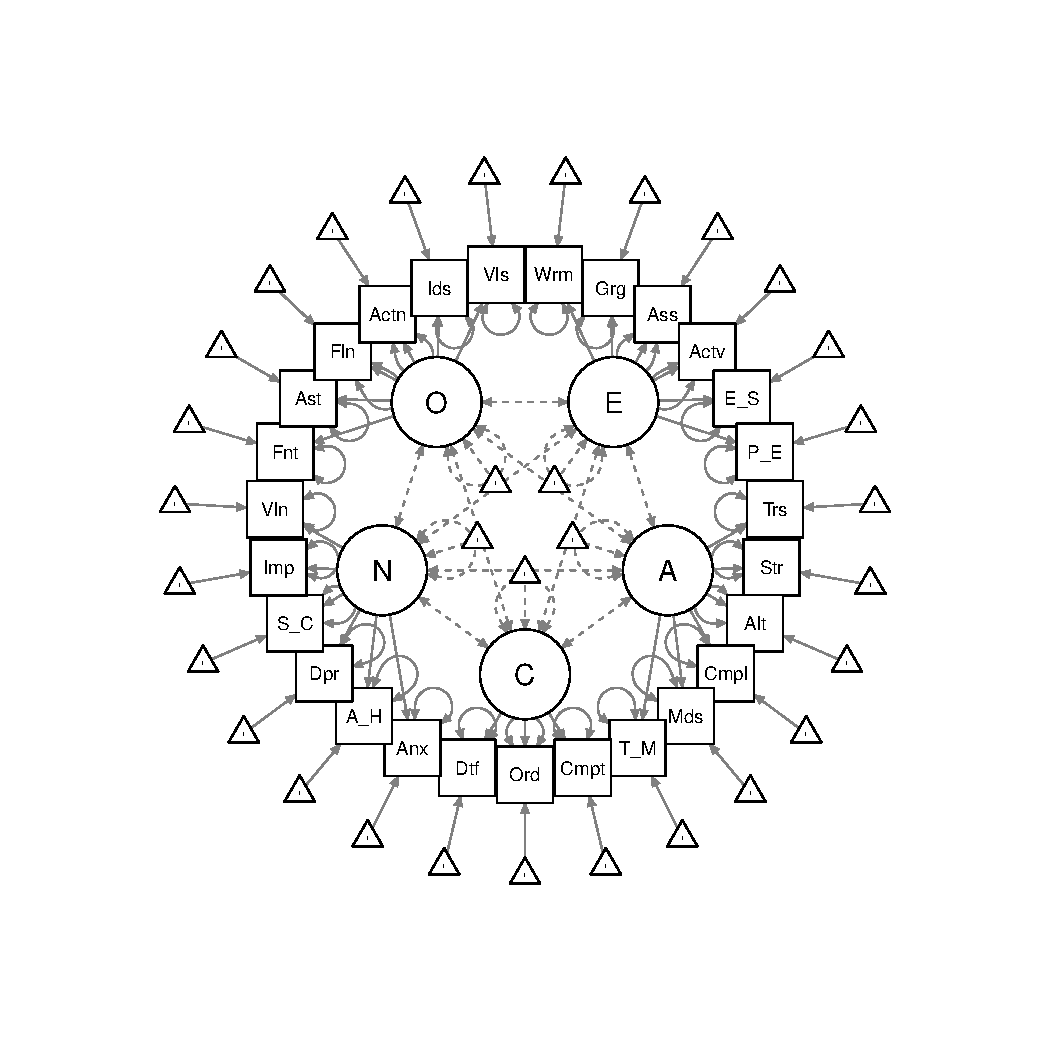
\includegraphics[width=\maxwidth]{figure/unnamed-chunk-5-1} 

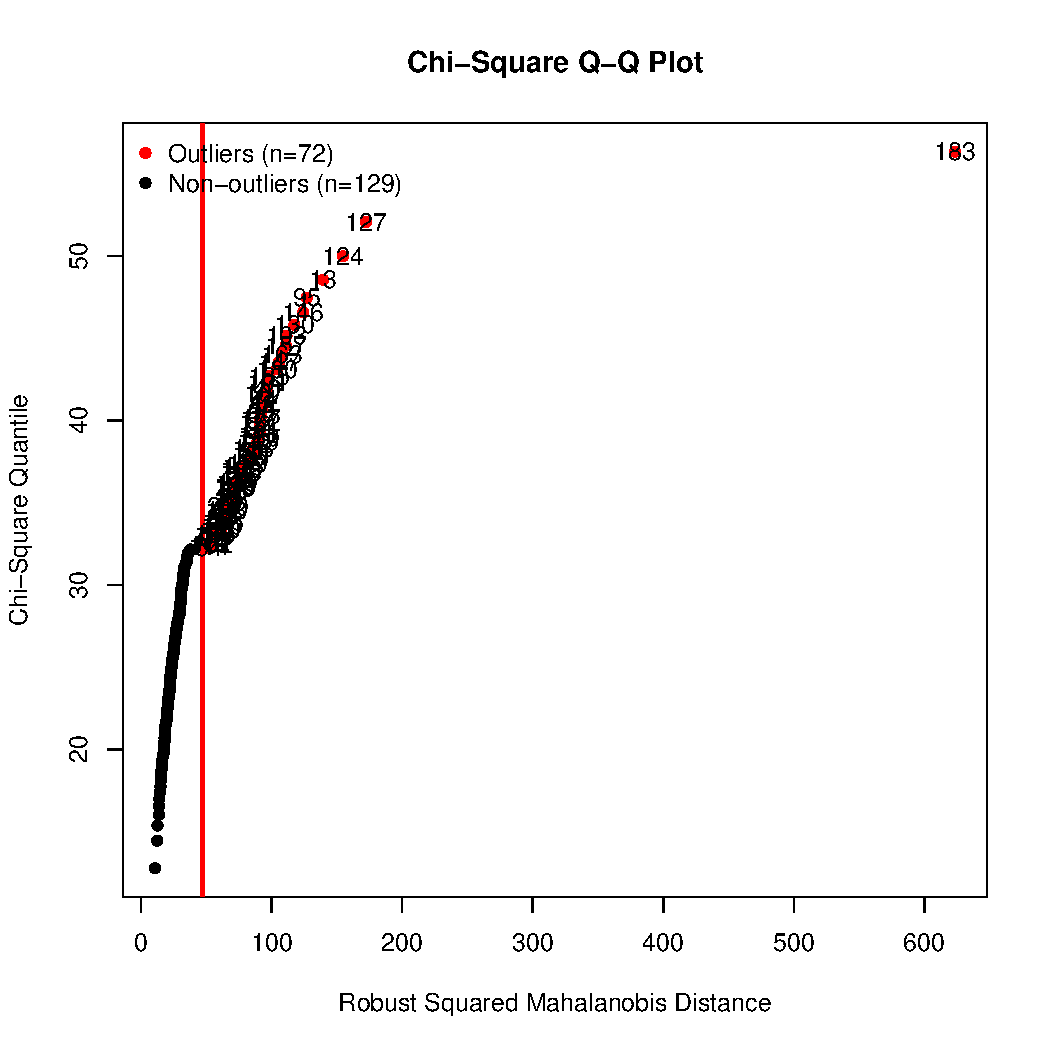
\includegraphics[width=\maxwidth]{figure/unnamed-chunk-5-2} 
\begin{kframe}\begin{verbatim}
## $multivariateNormality
##              Test        Statistic               p value Result
## 1 Mardia Skewness  8953.5001026237 9.27843696584267e-234     NO
## 2 Mardia Kurtosis 25.6787714020441                     0     NO
## 3             MVN             <NA>                  <NA>     NO
## 
## $univariateNormality
##            Test             Variable Statistic   p value Normality
## 1  Shapiro-Wilk       Anxiety           0.9688   2e-04      NO    
## 2  Shapiro-Wilk   Angry_Hostility       0.9826  0.0138      NO    
## 3  Shapiro-Wilk      Depression         0.9869  0.0595      YES   
## 4  Shapiro-Wilk  Self_Consciousness     0.9777  0.0028      NO    
## 5  Shapiro-Wilk    Impulsiveness        0.9472  <0.001      NO    
## 6  Shapiro-Wilk    Vulnerability        0.9857  0.0391      NO    
## 7  Shapiro-Wilk        Warmth           0.9344  <0.001      NO    
## 8  Shapiro-Wilk    Gregariousness       0.9785  0.0036      NO    
## 9  Shapiro-Wilk    Assertiveness        0.9839  0.0211      NO    
## 10 Shapiro-Wilk       Activity          0.9547  <0.001      NO    
## 11 Shapiro-Wilk  Excitement_Seeking     0.9499  <0.001      NO    
## 12 Shapiro-Wilk  Positive_Emotions      0.9491  <0.001      NO    
## 13 Shapiro-Wilk       Fantasy           0.9523  <0.001      NO    
## 14 Shapiro-Wilk      Aesthetics         0.9735   7e-04      NO    
## 15 Shapiro-Wilk       Feelings          0.9154  <0.001      NO    
## 16 Shapiro-Wilk       Actions           0.9627  <0.001      NO    
## 17 Shapiro-Wilk        Ideas            0.9696   2e-04      NO    
## 18 Shapiro-Wilk        Values           0.9087  <0.001      NO    
## 19 Shapiro-Wilk        Trust            0.9527  <0.001      NO    
## 20 Shapiro-Wilk Straightforwardness     0.9687   2e-04      NO    
## 21 Shapiro-Wilk       Altruism          0.9090  <0.001      NO    
## 22 Shapiro-Wilk      Compliance         0.9673   1e-04      NO    
## 23 Shapiro-Wilk       Modesty           0.9718   5e-04      NO    
## 24 Shapiro-Wilk  Tender_Mindedness      0.9164  <0.001      NO    
## 25 Shapiro-Wilk      Competence         0.9493  <0.001      NO    
## 26 Shapiro-Wilk        Order            0.9827  0.0143      NO    
## 27 Shapiro-Wilk     Dutifulness         0.9525  <0.001      NO    
## 28 Shapiro-Wilk Achievement_Striving    0.9609  <0.001      NO    
## 29 Shapiro-Wilk   Self_Discipline       0.9774  0.0025      NO    
## 30 Shapiro-Wilk     Deliberation        0.9615  <0.001      NO    
## 
## $Descriptives
##                        n     Mean   Std.Dev Median Min      Max     25th
## Anxiety              201 3.384453 0.7779526  3.500   0 4.875000 2.875000
## Angry_Hostility      201 2.821660 0.6890159  2.750   0 4.500000 2.375000
## Depression           201 2.949893 0.8391123  3.000   0 5.000000 2.375000
## Self_Consciousness   201 3.110519 0.6671846  3.125   0 4.750000 2.714286
## Impulsiveness        201 3.249556 0.5953863  3.375   0 4.625000 2.875000
## Vulnerability        201 2.609660 0.6780842  2.625   0 4.625000 2.125000
## Warmth               201 3.779561 0.6598163  3.875   0 5.000000 3.500000
## Gregariousness       201 3.158333 0.7554524  3.250   0 4.875000 2.750000
## Assertiveness        201 2.941927 0.7141767  3.000   0 4.875000 2.500000
## Activity             201 3.229004 0.5767897  3.250   0 4.833333 2.875000
## Excitement_Seeking   201 3.584577 0.6270903  3.625   0 5.000000 3.250000
## Positive_Emotions    201 3.684287 0.7378122  3.750   0 5.000000 3.125000
## Fantasy              201 3.659737 0.7265031  3.750   0 4.875000 3.250000
## Aesthetics           201 3.363539 0.8571747  3.375   0 5.000000 2.875000
## Feelings             201 3.887379 0.6477835  4.000   0 5.000000 3.500000
## Actions              201 2.971251 0.5849788  3.000   0 4.625000 2.625000
## Ideas                201 3.513599 0.7696339  3.625   0 5.000000 3.000000
## Values               201 3.783807 0.5664002  3.750   0 4.875000 3.500000
## Trust                201 3.343106 0.6984903  3.500   0 5.000000 3.000000
## Straightforwardness  201 3.247631 0.6981927  3.250   0 4.714286 2.750000
## Altruism             201 3.897092 0.5879144  3.875   0 5.000000 3.625000
## Compliance           201 3.114641 0.6383796  3.125   0 4.625000 2.750000
## Modesty              201 3.160537 0.6504879  3.250   0 5.000000 2.750000
## Tender_Mindedness    201 3.511058 0.5400171  3.500   0 4.800000 3.250000
## Competence           201 3.486407 0.6072013  3.500   0 5.000000 3.125000
## Order                201 3.165689 0.7473491  3.250   0 5.000000 2.625000
## Dutifulness          201 3.630360 0.6517670  3.625   0 5.000000 3.250000
## Achievement_Striving 201 3.371150 0.6828271  3.375   0 4.750000 3.000000
## Self_Discipline      201 3.261443 0.7019657  3.250   0 5.000000 2.875000
## Deliberation         201 3.106965 0.6145893  3.125   0 4.875000 2.750000
##                       75th        Skew   Kurtosis
## Anxiety              3.875 -0.65520717  0.8494755
## Angry_Hostility      3.250 -0.11418960  0.5226148
## Depression           3.500 -0.02546588 -0.1581829
## Self_Consciousness   3.500 -0.39666446  1.4360305
## Impulsiveness        3.625 -1.00765416  3.8124686
## Vulnerability        3.000  0.02402429  0.8095776
## Warmth               4.250 -1.16223708  4.2653957
## Gregariousness       3.625 -0.48949185  0.9682252
## Assertiveness        3.500 -0.37114794  0.5705680
## Activity             3.625 -0.80844019  3.8700815
## Excitement_Seeking   4.000 -0.95293496  4.2442910
## Positive_Emotions    4.125 -0.90030645  2.2648330
## Fantasy              4.250 -0.88404796  2.1427595
## Aesthetics           4.000 -0.63342270  0.5954302
## Feelings             4.375 -1.42084843  5.8519983
## Actions              3.375 -0.27038758  2.5855684
## Ideas                4.000 -0.61785669  1.3204615
## Values               4.125 -1.52503915  8.6067997
## Trust                3.750 -0.91355637  2.0762294
## Straightforwardness  3.750 -0.64260256  1.7225889
## Altruism             4.250 -1.54955211  8.2271156
## Compliance           3.625 -0.73499044  1.9911054
## Modesty              3.500 -0.58692618  2.2146126
## Tender_Mindedness    3.875 -1.49527616  7.7506175
## Competence           3.875 -0.87987169  4.3566406
## Order                3.625 -0.42211638  0.7859926
## Dutifulness          4.000 -0.86187907  3.7620876
## Achievement_Striving 3.750 -0.74643750  2.2765782
## Self_Discipline      3.750 -0.52501450  1.4461432
## Deliberation         3.500 -0.77452947  2.7793545
## 
## $multivariateOutliers
##     Observation Mahalanobis Distance Outlier
## 183         183              659.678    TRUE
## 127         127              167.071    TRUE
## 124         124              161.143    TRUE
## 13           13              151.489    TRUE
## 130         130              122.773    TRUE
## 95           95              119.521    TRUE
## 157         157              115.901    TRUE
## 146         146              115.801    TRUE
## 163         163              115.350    TRUE
## 103         103              113.642    TRUE
## 180         180              108.203    TRUE
## 147         147              106.359    TRUE
## 132         132               98.741    TRUE
## 167         167               98.056    TRUE
## 150         150               97.320    TRUE
## 62           62               96.021    TRUE
## 94           94               95.148    TRUE
## 185         185               92.874    TRUE
## 118         118               91.402    TRUE
## 113         113               90.491    TRUE
## 101         101               90.325    TRUE
## 177         177               90.167    TRUE
## 60           60               90.032    TRUE
## 105         105               88.414    TRUE
## 84           84               87.534    TRUE
## 40           40               87.376    TRUE
## 44           44               86.625    TRUE
## 182         182               85.756    TRUE
## 24           24               84.211    TRUE
## 2             2               84.114    TRUE
## 151         151               83.943    TRUE
## 46           46               82.738    TRUE
## 45           45               82.185    TRUE
## 90           90               80.278    TRUE
## 176         176               78.757    TRUE
## 42           42               78.028    TRUE
## 179         179               77.561    TRUE
## 121         121               76.356    TRUE
## 51           51               76.188    TRUE
## 25           25               73.157    TRUE
## 143         143               72.663    TRUE
## 190         190               72.155    TRUE
## 119         119               71.332    TRUE
## 120         120               70.421    TRUE
## 145         145               69.898    TRUE
## 93           93               68.914    TRUE
## 83           83               68.726    TRUE
## 18           18               68.433    TRUE
## 41           41               68.072    TRUE
## 7             7               67.741    TRUE
## 168         168               67.683    TRUE
## 200         200               67.166    TRUE
## 17           17               67.056    TRUE
## 11           11               67.013    TRUE
## 70           70               66.905    TRUE
## 144         144               66.595    TRUE
## 27           27               66.336    TRUE
## 43           43               64.412    TRUE
## 55           55               63.449    TRUE
## 117         117               63.067    TRUE
## 31           31               62.729    TRUE
## 74           74               61.775    TRUE
## 92           92               61.518    TRUE
## 64           64               61.073    TRUE
## 134         134               60.150    TRUE
## 30           30               58.706    TRUE
## 129         129               57.333    TRUE
## 3             3               56.163    TRUE
## 165         165               52.006    TRUE
## 82           82               51.205    TRUE
## 69           69               50.503    TRUE
## 38           38               48.784    TRUE
\end{verbatim}
\begin{alltt}
\hlstd{remove} \hlkwb{<-} \hlkwd{as.numeric}\hlstd{(}\hlkwd{as.character}\hlstd{(mv}\hlopt{$}\hlstd{multivariateOutliers}\hlopt{$}\hlstd{Observation[}\hlnum{1}\hlstd{]))}
\hlstd{dat2} \hlkwb{<-} \hlstd{dat} \hlopt \hlkwd{filter}\hlstd{(}\hlopt{!}\hlstd{(ID} \hlopt \hlstd{remove))}
\end{alltt}
\end{kframe}
\end{knitrout}


Use confirmatory factor analysis to answer the following questions.  

\section{Question 1}
First, test the hypothesis that the structure of personality is best described by five independent factors. How well does this model fit the data? Base your decision on the $\chi^2$ goodness of fit test along with the goodness-of-fit index of your choice.  
\begin{knitrout}
\definecolor{shadecolor}{rgb}{0.969, 0.969, 0.969}\color{fgcolor}\begin{kframe}
\begin{alltt}
\hlstd{b5.base} \hlkwb{<-} \hlstr{'
# define the measurement model
E =~ Warmth + Gregariousness + Assertiveness + Activity + Excitement_Seeking + Positive_Emotions
A =~ Trust + Straightforwardness + Altruism + Compliance + Modesty + Tender_Mindedness
C =~ Competence + Order + Dutifulness + Competence + Order + Dutifulness
N =~ Anxiety + Angry_Hostility + Depression + Self_Consciousness + Impulsiveness + Vulnerability
O =~ Fantasy + Aesthetics + Feelings + Actions + Ideas + Values
'}
\hlstd{b5.uncorr} \hlkwb{<-}
\hlstr{'
# uncorrelated factors
E ~~ 0*A
E ~~ 0*C
E ~~ 0*N
E ~~ 0*O

A ~~ 0*C
A ~~ 0*N
A ~~ 0*O

C ~~ 0*N
C ~~ 0*O
'}

\hlstd{b5.mod} \hlkwb{<-} \hlkwd{paste}\hlstd{(b5.base,} \hlstr{'\textbackslash{}n\textbackslash{}n'}\hlstd{, b5.uncorr,} \hlkwc{sep} \hlstd{=} \hlstr{''}\hlstd{,} \hlkwc{collapse} \hlstd{=} \hlstr{''}\hlstd{)}

\hlstd{fit1} \hlkwb{<-} \hlkwd{cfa}\hlstd{(b5.mod, dat2,} \hlkwc{orthogonal} \hlstd{= T,} \hlkwc{missing} \hlstd{=} \hlstr{'ML'}\hlstd{,} \hlkwc{std.lv} \hlstd{= T)}

\hlkwd{semPaths}\hlstd{(fit1,} \hlkwc{layout} \hlstd{=} \hlstr{"circle2"}\hlstd{)}
\end{alltt}
\end{kframe}
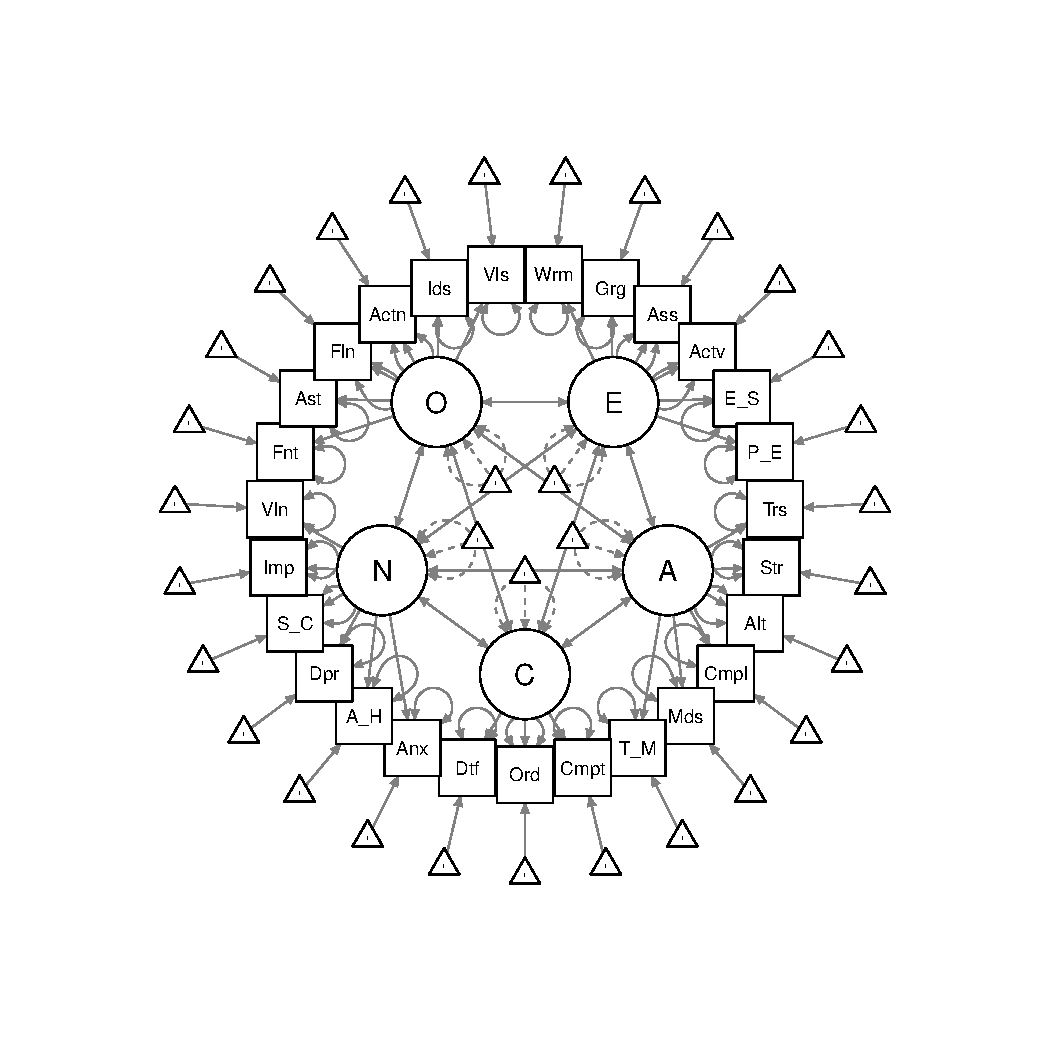
\includegraphics[width=\maxwidth]{figure/unnamed-chunk-6-1} 
\begin{kframe}\begin{alltt}
\hlkwd{summary}\hlstd{(fit1)}
\end{alltt}
\begin{verbatim}
## lavaan 0.6-3 ended normally after 54 iterations
## 
##   Optimization method                           NLMINB
##   Number of free parameters                         81
## 
##   Number of observations                           200
##   Number of missing patterns                         1
## 
##   Estimator                                         ML
##   Model Fit Test Statistic                    1412.317
##   Degrees of freedom                               324
##   P-value (Chi-square)                           0.000
## 
## Parameter Estimates:
## 
##   Information                                 Observed
##   Observed information based on                Hessian
##   Standard Errors                             Standard
## 
## Latent Variables:
##                    Estimate  Std.Err  z-value  P(>|z|)
##   E =~                                                
##     Warmth            0.464    0.040   11.706    0.000
##     Gregariousness    0.518    0.049   10.614    0.000
##     Assertiveness     0.364    0.049    7.402    0.000
##     Activity          0.293    0.038    7.723    0.000
##     Excitemnt_Skng    0.248    0.043    5.783    0.000
##     Positive_Emtns    0.522    0.046   11.449    0.000
##   A =~                                                
##     Trust             0.403    0.050    8.138    0.000
##     Strghtfrwrdnss    0.359    0.051    7.058    0.000
##     Altruism          0.348    0.039    8.978    0.000
##     Compliance        0.358    0.045    7.887    0.000
##     Modesty           0.255    0.049    5.240    0.000
##     Tender_Mnddnss    0.244    0.037    6.594    0.000
##   C =~                                                
##     Competence        0.394    0.042    9.363    0.000
##     Order             0.449    0.053    8.424    0.000
##     Dutifulness       0.464    0.046   10.091    0.000
##   N =~                                                
##     Anxiety           0.614    0.045   13.703    0.000
##     Angry_Hostilty    0.323    0.046    6.995    0.000
##     Depression        0.695    0.048   14.390    0.000
##     Self_Conscsnss    0.471    0.040   11.863    0.000
##     Impulsiveness     0.213    0.040    5.392    0.000
##     Vulnerability     0.516    0.040   12.895    0.000
##   O =~                                                
##     Fantasy           0.444    0.051    8.675    0.000
##     Aesthetics        0.528    0.063    8.432    0.000
##     Feelings          0.282    0.046    6.173    0.000
##     Actions           0.303    0.042    7.209    0.000
##     Ideas             0.350    0.057    6.123    0.000
##     Values            0.287    0.038    7.603    0.000
## 
## Covariances:
##                    Estimate  Std.Err  z-value  P(>|z|)
##   E ~~                                                
##     A                 0.000                           
##     C                 0.000                           
##     N                 0.000                           
##     O                 0.000                           
##   A ~~                                                
##     C                 0.000                           
##     N                 0.000                           
##     O                 0.000                           
##   C ~~                                                
##     N                 0.000                           
##     O                 0.000                           
##   N ~~                                                
##     O                 0.000                           
## 
## Intercepts:
##                    Estimate  Std.Err  z-value  P(>|z|)
##    .Warmth            3.798    0.043   89.089    0.000
##    .Gregariousness    3.174    0.051   62.215    0.000
##    .Assertiveness     2.957    0.048   61.215    0.000
##    .Activity          3.245    0.037   86.685    0.000
##    .Excitemnt_Skng    3.603    0.041   88.866    0.000
##    .Positive_Emtns    3.703    0.049   75.886    0.000
##    .Trust             3.360    0.046   72.315    0.000
##    .Strghtfrwrdnss    3.264    0.047   70.027    0.000
##    .Altruism          3.917    0.037  106.729    0.000
##    .Compliance        3.130    0.042   73.905    0.000
##    .Modesty           3.176    0.043   73.557    0.000
##    .Tender_Mnddnss    3.529    0.034  104.127    0.000
##    .Competence        3.504    0.039   89.342    0.000
##    .Order             3.182    0.050   63.117    0.000
##    .Dutifulness       3.649    0.042   86.167    0.000
##    .Anxiety           3.401    0.052   65.001    0.000
##    .Angry_Hostilty    2.836    0.047   60.824    0.000
##    .Depression        2.965    0.057   51.593    0.000
##    .Self_Conscsnss    3.126    0.045   70.207    0.000
##    .Impulsiveness     3.266    0.039   84.123    0.000
##    .Vulnerability     2.623    0.046   56.856    0.000
##    .Fantasy           3.678    0.048   76.650    0.000
##    .Aesthetics        3.380    0.058   58.062    0.000
##    .Feelings          3.907    0.041   94.244    0.000
##    .Actions           2.986    0.039   77.380    0.000
##    .Ideas             3.531    0.051   68.576    0.000
##    .Values            3.803    0.035  107.802    0.000
##     E                 0.000                           
##     A                 0.000                           
##     C                 0.000                           
##     N                 0.000                           
##     O                 0.000                           
## 
## Variances:
##                    Estimate  Std.Err  z-value  P(>|z|)
##    .Warmth            0.149    0.022    6.862    0.000
##    .Gregariousness    0.252    0.033    7.556    0.000
##    .Assertiveness     0.334    0.037    9.149    0.000
##    .Activity          0.194    0.022    9.006    0.000
##    .Excitemnt_Skng    0.267    0.028    9.457    0.000
##    .Positive_Emtns    0.203    0.029    7.043    0.000
##    .Trust             0.269    0.034    7.848    0.000
##    .Strghtfrwrdnss    0.305    0.036    8.425    0.000
##    .Altruism          0.148    0.021    7.031    0.000
##    .Compliance        0.231    0.029    8.001    0.000
##    .Modesty           0.308    0.033    9.199    0.000
##    .Tender_Mnddnss    0.170    0.019    8.771    0.000
##    .Competence        0.153    0.025    6.160    0.000
##    .Order             0.307    0.040    7.702    0.000
##    .Dutifulness       0.144    0.031    4.686    0.000
##    .Anxiety           0.171    0.025    6.946    0.000
##    .Angry_Hostilty    0.330    0.034    9.603    0.000
##    .Depression        0.177    0.028    6.383    0.000
##    .Self_Conscsnss    0.174    0.021    8.334    0.000
##    .Impulsiveness     0.256    0.026    9.773    0.000
##    .Vulnerability     0.159    0.020    7.908    0.000
##    .Fantasy           0.263    0.037    7.202    0.000
##    .Aesthetics        0.399    0.054    7.340    0.000
##    .Feelings          0.264    0.030    8.924    0.000
##    .Actions           0.206    0.025    8.355    0.000
##    .Ideas             0.408    0.046    8.857    0.000
##    .Values            0.166    0.020    8.255    0.000
##     E                 1.000                           
##     A                 1.000                           
##     C                 1.000                           
##     N                 1.000                           
##     O                 1.000
\end{verbatim}
\begin{alltt}
\hlstd{fm} \hlkwb{<-} \hlkwd{fitmeasures}\hlstd{(fit1)}
\end{alltt}
\end{kframe}
\end{knitrout}

The $\chi^2$ test indicates poor model fit, $\chi^2(324) = 1412.32, p = 0$. 


\section{Question 2}
Now allow the factors to correlate.  

\subsection{Part A}
Does this model fit the data significantly better? Use a $\chi^2$ difference test to answer the question.

\begin{knitrout}
\definecolor{shadecolor}{rgb}{0.969, 0.969, 0.969}\color{fgcolor}\begin{kframe}
\begin{alltt}
\hlstd{fit2} \hlkwb{<-} \hlkwd{cfa}\hlstd{(b5.base, dat2,} \hlkwc{missing} \hlstd{=} \hlstr{'ML'}\hlstd{,} \hlkwc{std.lv} \hlstd{= T)}
\hlkwd{semPaths}\hlstd{(fit2,} \hlkwc{layout} \hlstd{=} \hlstr{"circle2"}\hlstd{)}
\end{alltt}
\end{kframe}
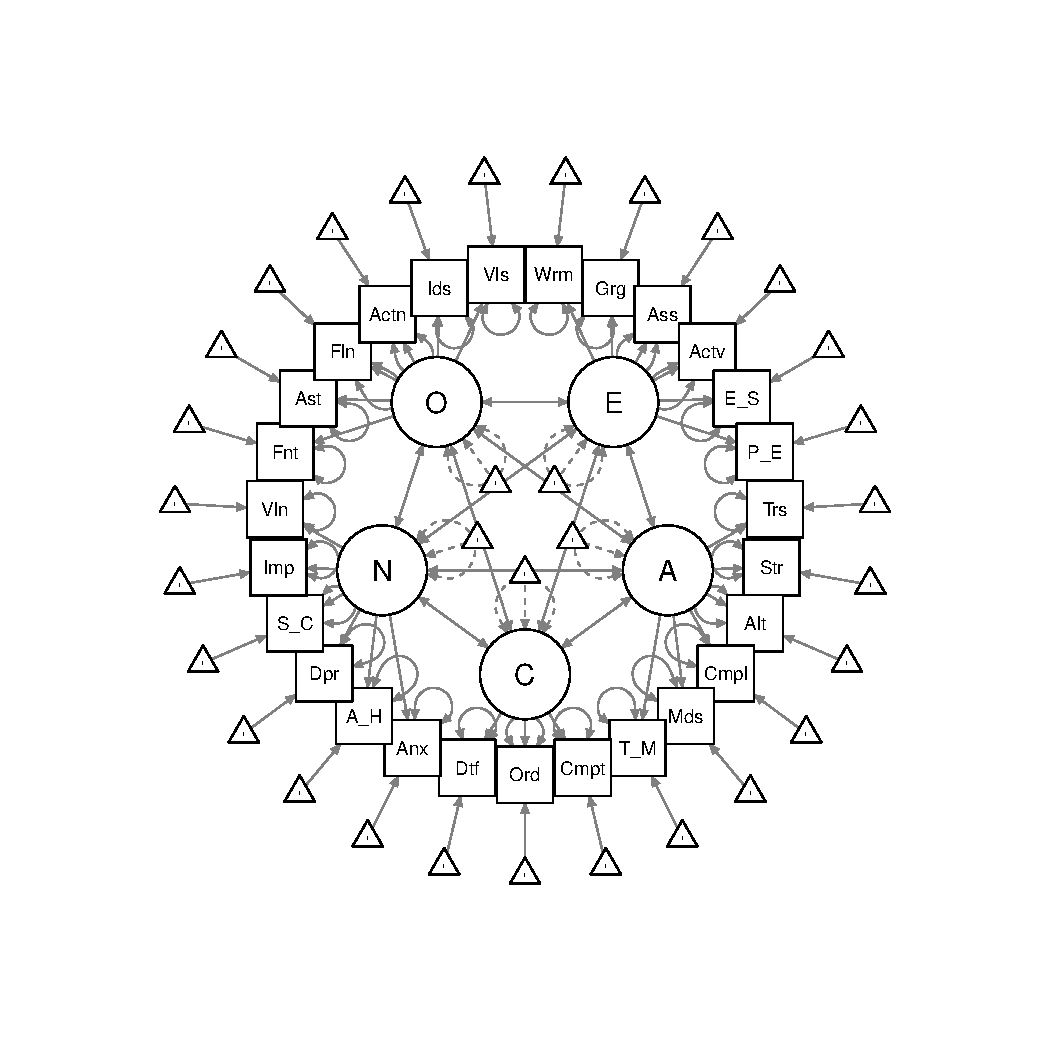
\includegraphics[width=\maxwidth]{figure/unnamed-chunk-7-1} 
\begin{kframe}\begin{alltt}
\hlstd{(c1} \hlkwb{<-} \hlkwd{anova}\hlstd{(fit1, fit2))}
\end{alltt}
\begin{verbatim}
## Chi Square Difference Test
## 
##       Df    AIC    BIC  Chisq Chisq diff Df diff Pr(>Chisq)    
## fit2 314 8964.5 9264.6 1261.2                                  
## fit1 324 9095.6 9362.8 1412.3     151.14      10  < 2.2e-16 ***
## ---
## Signif. codes:  0 '***' 0.001 '**' 0.01 '*' 0.05 '.' 0.1 ' ' 1
\end{verbatim}
\end{kframe}
\end{knitrout}

The correlated factor model fits the data better, $\chi^2_{diff}(10) = 151.14$. 

\subsection{Part B}
Which of the factor correlations are statistically significant?  
\begin{knitrout}
\definecolor{shadecolor}{rgb}{0.969, 0.969, 0.969}\color{fgcolor}\begin{kframe}
\begin{alltt}
\hlstd{res2} \hlkwb{<-} \hlkwd{parameterestimates}\hlstd{(fit2,} \hlkwc{standardized} \hlstd{= T)}

\hlstd{res2} \hlopt \hlstd{tbl_df} \hlopt
  \hlkwd{filter}\hlstd{(op} \hlopt{==} \hlstr{"~~"} \hlopt{&} \hlstd{lhs} \hlopt \hlkwd{c}\hlstd{(}\hlstr{"E"}\hlstd{,} \hlstr{"A"}\hlstd{,} \hlstr{"C"}\hlstd{,} \hlstr{"N"}\hlstd{,} \hlstr{"O"}\hlstd{))} \hlopt
  \hlkwd{full_join}\hlstd{(}\hlkwd{crossing}\hlstd{(}\hlkwc{lhs} \hlstd{=} \hlkwd{c}\hlstd{(}\hlstr{"E"}\hlstd{,} \hlstr{"A"}\hlstd{,} \hlstr{"C"}\hlstd{,} \hlstr{"N"}\hlstd{,} \hlstr{"O"}\hlstd{),} \hlkwc{rhs} \hlstd{=} \hlkwd{c}\hlstd{(}\hlstr{"E"}\hlstd{,} \hlstr{"A"}\hlstd{,} \hlstr{"C"}\hlstd{,} \hlstr{"N"}\hlstd{,} \hlstr{"O"}\hlstd{)))} \hlopt
  \hlkwd{mutate}\hlstd{(}\hlkwc{sig} \hlstd{=} \hlkwd{ifelse}\hlstd{(pvalue} \hlopt{<} \hlnum{.05}\hlstd{,} \hlstr{"sig"}\hlstd{,} \hlstr{"ns"}\hlstd{))} \hlopt
  \hlkwd{select}\hlstd{(lhs, rhs, est, ci.lower, ci.upper, sig)} \hlopt
  \hlkwd{mutate_at}\hlstd{(}\hlkwd{vars}\hlstd{(est}\hlopt{:}\hlstd{ci.upper),} \hlkwd{funs}\hlstd{(}\hlkwd{sprintf}\hlstd{(}\hlstr{"%.2f"}\hlstd{, .)))} \hlopt
  \hlkwd{mutate_at}\hlstd{(}\hlkwd{vars}\hlstd{(lhs, rhs),} \hlkwd{funs}\hlstd{(}\hlkwd{factor}\hlstd{(.,} \hlkwc{levels} \hlstd{=} \hlkwd{c}\hlstd{(}\hlstr{"E"}\hlstd{,} \hlstr{"A"}\hlstd{,} \hlstr{"C"}\hlstd{,} \hlstr{"N"}\hlstd{,} \hlstr{"O"}\hlstd{))))} \hlopt
  \hlkwd{mutate}\hlstd{(}\hlkwc{value} \hlstd{=} \hlkwd{sprintf}\hlstd{(}\hlstr{"%s [%s, %s]"}\hlstd{, est, ci.lower, ci.upper),}
         \hlkwc{value} \hlstd{=} \hlkwd{ifelse}\hlstd{(sig} \hlopt{==} \hlstr{"sig"}\hlstd{,} \hlkwd{sprintf}\hlstd{(}\hlstr{"\textbackslash{}\textbackslash{}textbf\{%s\}"}\hlstd{, value), value),}
         \hlkwc{value} \hlstd{=} \hlkwd{ifelse}\hlstd{(}\hlkwd{is.na}\hlstd{(value),} \hlstr{""}\hlstd{, value))} \hlopt
  \hlkwd{select}\hlstd{(lhs, rhs, value)} \hlopt
  \hlkwd{spread}\hlstd{(}\hlkwc{key} \hlstd{= rhs,} \hlkwc{value} \hlstd{= value)} \hlopt
  \hlkwd{kable}\hlstd{(.,} \hlstr{"latex"}\hlstd{,} \hlkwc{booktabs} \hlstd{= T,} \hlkwc{escape} \hlstd{= F,}
        \hlkwc{caption} \hlstd{=} \hlstr{"Question 2B"}\hlstd{)} \hlopt
  \hlkwd{kable_styling}\hlstd{(}\hlkwc{full_width} \hlstd{= F)}
\end{alltt}
\end{kframe}\begin{table}

\caption{\label{tab:unnamed-chunk-8}Question 2B}
\centering
\begin{tabular}[t]{llllll}
\toprule
lhs & E & A & C & N & O\\
\midrule
E &  & \textbf{0.60 [0.46, 0.74]} & \textbf{0.34 [0.17, 0.51]} & \textbf{-0.41 [-0.55, -0.28]} & \textbf{0.46 [0.30, 0.62]}\\
A &  &  & \textbf{0.32 [0.15, 0.49]} & 0.01 [-0.17, 0.18] & \textbf{0.31 [0.14, 0.48]}\\
C &  &  &  & \textbf{-0.32 [-0.53, -0.12]} & \textbf{-0.26 [-0.45, -0.07]}\\
N &  &  &  &  & -0.03 [-0.21, 0.14]\\
O &  &  &  &  & \\
\bottomrule
\end{tabular}
\end{table}


\end{knitrout}

\section{Question 3}
Test a model that constrains all factor correlations to be equal.  
\begin{knitrout}
\definecolor{shadecolor}{rgb}{0.969, 0.969, 0.969}\color{fgcolor}\begin{kframe}
\begin{alltt}
\hlstd{b5.corr} \hlkwb{<-} \hlstr{'
# equally correlated factors
E ~~ lambda*A
E ~~ lambda*C
E ~~ lambda*N
E ~~ lambda*O

A ~~ lambda*C
A ~~ lambda*N
A ~~ lambda*O

C ~~ lambda*N
C ~~ lambda*O
'}

\hlstd{b5.mod} \hlkwb{<-} \hlkwd{paste}\hlstd{(b5.base,} \hlstr{'\textbackslash{}n\textbackslash{}n'}\hlstd{, b5.corr,} \hlkwc{sep} \hlstd{=} \hlstr{''}\hlstd{,} \hlkwc{collapse} \hlstd{=} \hlstr{''}\hlstd{)}
\hlstd{fit3} \hlkwb{<-} \hlkwd{cfa}\hlstd{(b5.mod, dat2,} \hlkwc{missing} \hlstd{=} \hlstr{'ML'}\hlstd{,} \hlkwc{std.lv} \hlstd{= T)}
\hlkwd{semPaths}\hlstd{(fit3,} \hlkwc{layout} \hlstd{=} \hlstr{"circle2"}\hlstd{)}
\end{alltt}
\end{kframe}
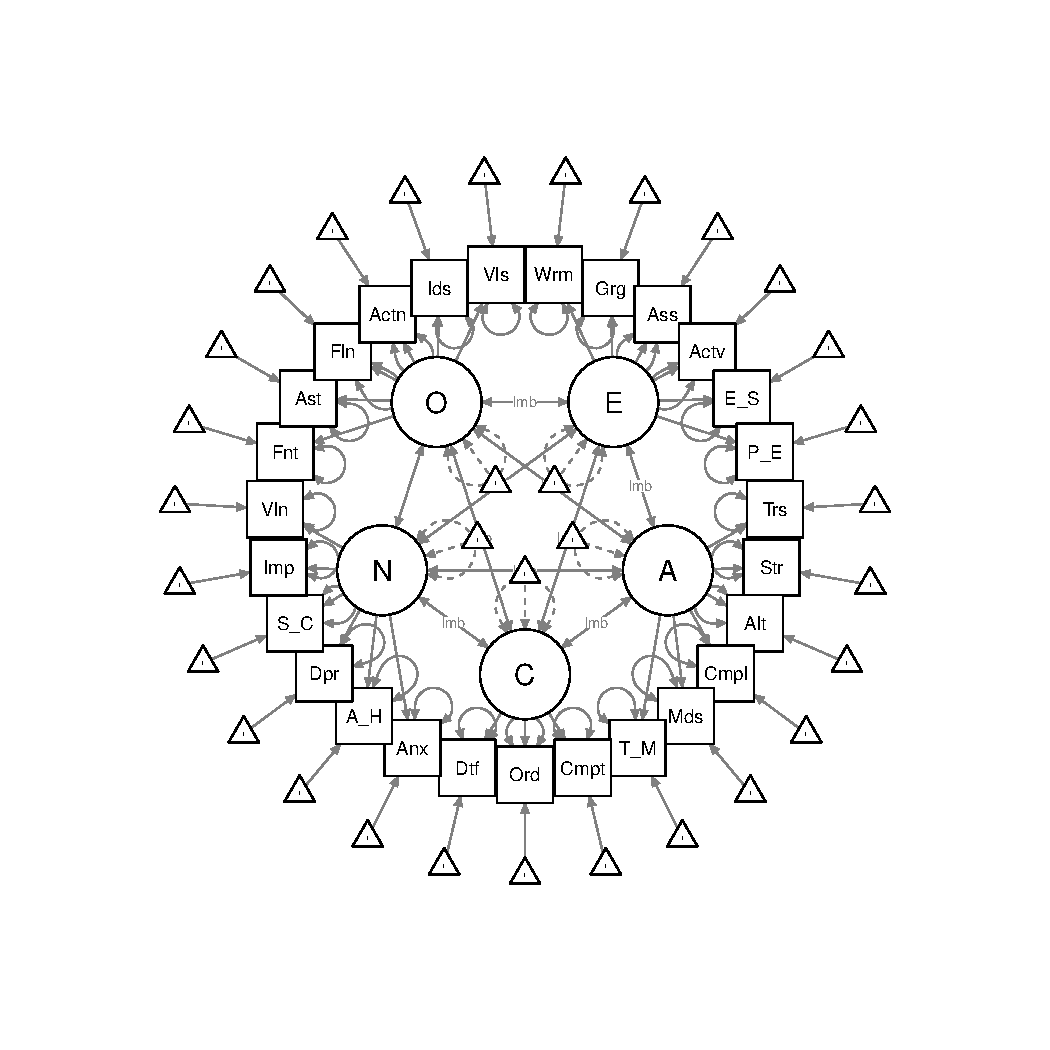
\includegraphics[width=\maxwidth]{figure/unnamed-chunk-9-1} 

\end{knitrout}

\subsection{Part A}
Is this constraint acceptable (i.e., is it statistically different from the model tested in Question 2)?
\begin{knitrout}
\definecolor{shadecolor}{rgb}{0.969, 0.969, 0.969}\color{fgcolor}\begin{kframe}
\begin{alltt}
\hlstd{(c3} \hlkwb{<-} \hlkwd{anova}\hlstd{(fit3, fit2))}
\end{alltt}
\begin{verbatim}
## Chi Square Difference Test
## 
##       Df    AIC    BIC  Chisq Chisq diff Df diff Pr(>Chisq)    
## fit2 314 8964.5 9264.6 1261.2                                  
## fit3 322 9092.4 9366.2 1405.1     143.97       8  < 2.2e-16 ***
## ---
## Signif. codes:  0 '***' 0.001 '**' 0.01 '*' 0.05 '.' 0.1 ' ' 1
\end{verbatim}
\end{kframe}
\end{knitrout}

Constraining the factor correlations to be equal does not appear to be justified, $\chi^2_{diff}(8) = 143.97$. 

\subsection{Part B}
Is the estimated latent variable correlation significant?

\begin{knitrout}
\definecolor{shadecolor}{rgb}{0.969, 0.969, 0.969}\color{fgcolor}\begin{kframe}
\begin{alltt}
\hlstd{res3} \hlkwb{<-} \hlkwd{parameterestimates}\hlstd{(fit3,} \hlkwc{standardized} \hlstd{= T)}

\hlstd{res3} \hlopt \hlstd{tbl_df} \hlopt \hlkwd{filter}\hlstd{(label} \hlopt{==} \hlstr{"lambda"}\hlstd{)} \hlopt
  \hlkwd{select}\hlstd{(label, est, ci.lower, ci.upper)} \hlopt
  \hlkwd{filter}\hlstd{(}\hlkwd{row_number}\hlstd{()} \hlopt{==} \hlnum{1}\hlstd{)}
\end{alltt}
\begin{verbatim}
## # A tibble: 1 x 4
##   label     est ci.lower ci.upper
##   <chr>   <dbl>    <dbl>    <dbl>
## 1 lambda 0.0834   0.0165    0.150
\end{verbatim}
\end{kframe}
\end{knitrout}

Yes, the estimated latent variable correlation is significant. 

\section{Question 4}
Use the most parsimonious model from the first three steps. Constrain the loadings within each dimension to be equal. Is this simplification acceptable?  

Fit 1 is the most parsimonious model because it estimates the fewest parameters.  

\begin{knitrout}
\definecolor{shadecolor}{rgb}{0.969, 0.969, 0.969}\color{fgcolor}\begin{kframe}
\begin{alltt}
\hlstd{b5.lc} \hlkwb{<-} \hlstr{'
# define the measurement model
E =~ lambdaE*Warmth + lambdaE*Gregariousness + lambdaE*Assertiveness + lambdaE*Activity + lambdaE*Excitement_Seeking + lambdaE*Positive_Emotions
A =~ lambdaA*Trust + lambdaA*Straightforwardness + lambdaA*Altruism + lambdaA*Compliance + lambdaA*Modesty + lambdaA*Tender_Mindedness
C =~ lambdaC*Competence + lambdaC*Order + lambdaC*Dutifulness + lambdaC*Competence + lambdaC*Order + lambdaC*Dutifulness
N =~ lambdaN*Anxiety + lambdaN*Angry_Hostility + lambdaN*Depression + lambdaN*Self_Consciousness + lambdaN*Impulsiveness + lambdaN*Vulnerability
O =~ lambdaO*Fantasy + lambdaO*Aesthetics + lambdaO*Feelings + lambdaO*Actions + lambdaO*Ideas + lambdaO*Values
'}

\hlstd{b5.mod} \hlkwb{<-} \hlkwd{paste}\hlstd{(b5.lc,} \hlstr{'\textbackslash{}n\textbackslash{}n'}\hlstd{, b5.uncorr,} \hlkwc{sep} \hlstd{=} \hlstr{''}\hlstd{,} \hlkwc{collapse} \hlstd{=} \hlstr{''}\hlstd{)}
\hlstd{fit4} \hlkwb{<-} \hlkwd{cfa}\hlstd{(b5.mod, dat2,} \hlkwc{missing} \hlstd{=} \hlstr{'ML'}\hlstd{,} \hlkwc{std.lv} \hlstd{= T)}
\hlkwd{semPaths}\hlstd{(fit4,} \hlkwc{layout} \hlstd{=} \hlstr{"circle2"}\hlstd{)}
\end{alltt}
\end{kframe}
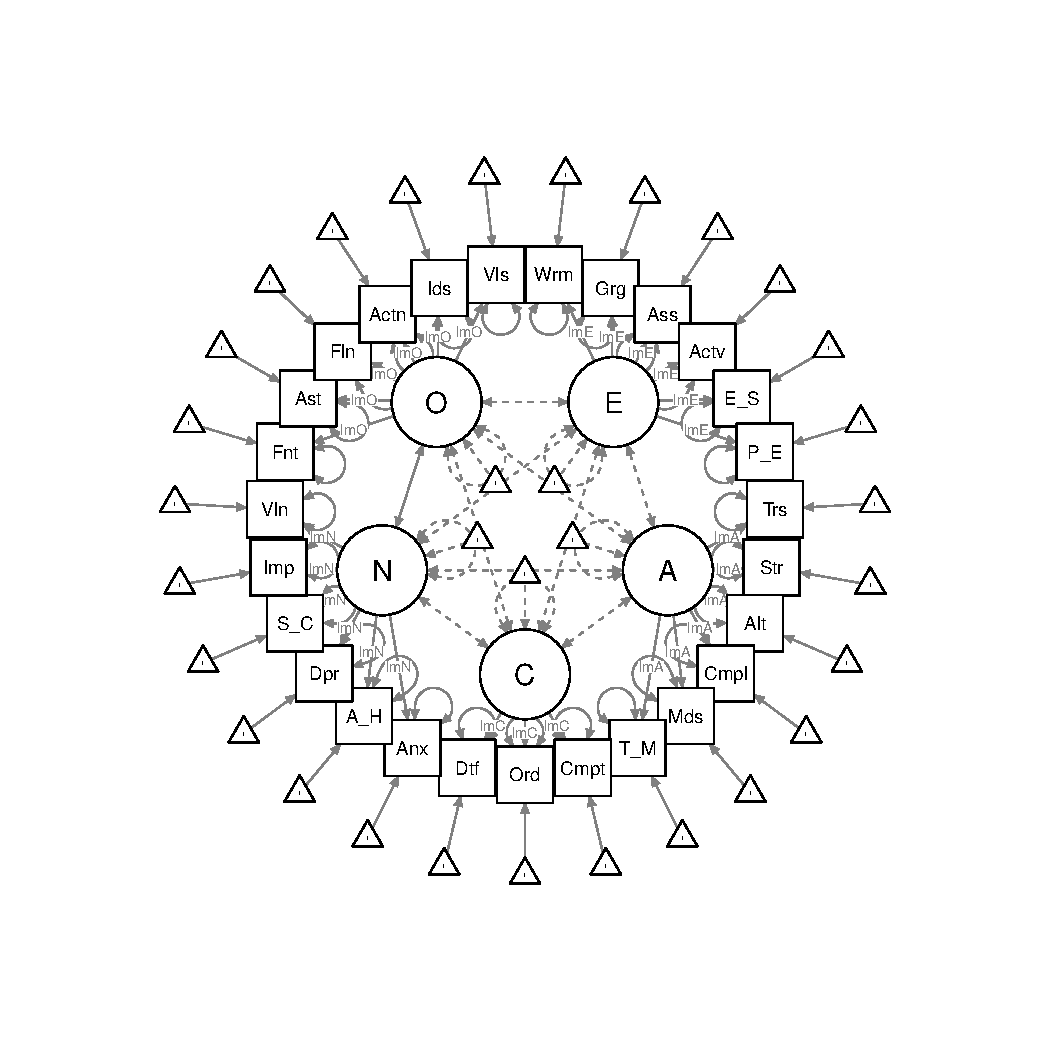
\includegraphics[width=\maxwidth]{figure/unnamed-chunk-12-1} 
\begin{kframe}\begin{alltt}
\hlkwd{summary}\hlstd{(fit4)}
\end{alltt}
\begin{verbatim}
## lavaan 0.6-3 ended normally after 63 iterations
## 
##   Optimization method                           NLMINB
##   Number of free parameters                         82
##   Number of equality constraints                    22
## 
##   Number of observations                           200
##   Number of missing patterns                         1
## 
##   Estimator                                         ML
##   Model Fit Test Statistic                    1597.946
##   Degrees of freedom                               345
##   P-value (Chi-square)                           0.000
## 
## Parameter Estimates:
## 
##   Information                                 Observed
##   Observed information based on                Hessian
##   Standard Errors                             Standard
## 
## Latent Variables:
##                    Estimate  Std.Err  z-value  P(>|z|)
##   E =~                                                
##     Warmth  (lmbE)    0.396    0.025   15.638    0.000
##     Grgrsns (lmbE)    0.396    0.025   15.638    0.000
##     Assrtvn (lmbE)    0.396    0.025   15.638    0.000
##     Activty (lmbE)    0.396    0.025   15.638    0.000
##     Exctm_S (lmbE)    0.396    0.025   15.638    0.000
##     Pstv_Em (lmbE)    0.396    0.025   15.638    0.000
##   A =~                                                
##     Trust   (lmbA)    0.321    0.022   14.507    0.000
##     Strghtf (lmbA)    0.321    0.022   14.507    0.000
##     Altrusm (lmbA)    0.321    0.022   14.507    0.000
##     Complnc (lmbA)    0.321    0.022   14.507    0.000
##     Modesty (lmbA)    0.321    0.022   14.507    0.000
##     Tndr_Mn (lmbA)    0.321    0.022   14.507    0.000
##   C =~                                                
##     Comptnc (lmbC)    0.431    0.029   14.871    0.000
##     Order   (lmbC)    0.431    0.029   14.871    0.000
##     Dtflnss (lmbC)    0.431    0.029   14.871    0.000
##   N =~                                                
##     Anxiety (lmbN)    0.486    0.029   16.641    0.000
##     Angry_H (lmbN)    0.486    0.029   16.641    0.000
##     Deprssn (lmbN)    0.486    0.029   16.641    0.000
##     Slf_Cns (lmbN)    0.486    0.029   16.641    0.000
##     Implsvn (lmbN)    0.486    0.029   16.641    0.000
##     Vlnrblt (lmbN)    0.486    0.029   16.641    0.000
##   O =~                                                
##     Fantasy (lmbO)    0.341    0.024   14.425    0.000
##     Asthtcs (lmbO)    0.341    0.024   14.425    0.000
##     Feelngs (lmbO)    0.341    0.024   14.425    0.000
##     Actions (lmbO)    0.341    0.024   14.425    0.000
##     Ideas   (lmbO)    0.341    0.024   14.425    0.000
##     Values  (lmbO)    0.341    0.024   14.425    0.000
## 
## Covariances:
##                    Estimate  Std.Err  z-value  P(>|z|)
##   E ~~                                                
##     A                 0.000                           
##     C                 0.000                           
##     N                 0.000                           
##     O                 0.000                           
##   A ~~                                                
##     C                 0.000                           
##     N                 0.000                           
##     O                 0.000                           
##   C ~~                                                
##     N                 0.000                           
##     O                 0.000                           
##   N ~~                                                
##     O                -0.050    0.090   -0.558    0.577
## 
## Intercepts:
##                    Estimate  Std.Err  z-value  P(>|z|)
##    .Warmth            3.798    0.041   92.146    0.000
##    .Gregariousness    3.174    0.047   67.696    0.000
##    .Assertiveness     2.957    0.049   60.478    0.000
##    .Activity          3.245    0.041   79.492    0.000
##    .Excitemnt_Skng    3.603    0.046   78.369    0.000
##    .Positive_Emtns    3.703    0.045   82.033    0.000
##    .Trust             3.360    0.045   74.882    0.000
##    .Strghtfrwrdnss    3.264    0.046   71.336    0.000
##    .Altruism          3.917    0.036  108.755    0.000
##    .Compliance        3.130    0.041   75.548    0.000
##    .Modesty           3.176    0.045   71.290    0.000
##    .Tender_Mnddnss    3.529    0.036   97.873    0.000
##    .Competence        3.504    0.040   87.573    0.000
##    .Order             3.182    0.050   63.712    0.000
##    .Dutifulness       3.649    0.042   87.427    0.000
##    .Anxiety           3.401    0.047   72.135    0.000
##    .Angry_Hostilty    2.836    0.053   53.347    0.000
##    .Depression        2.965    0.050   59.592    0.000
##    .Self_Conscsnss    3.126    0.046   68.506    0.000
##    .Impulsiveness     3.266    0.052   63.034    0.000
##    .Vulnerability     2.623    0.045   58.658    0.000
##    .Fantasy           3.678    0.045   81.125    0.000
##    .Aesthetics        3.380    0.055   61.924    0.000
##    .Feelings          3.907    0.044   89.404    0.000
##    .Actions           2.986    0.039   75.610    0.000
##    .Ideas             3.531    0.052   68.543    0.000
##    .Values            3.803    0.037  104.043    0.000
##     E                 0.000                           
##     A                 0.000                           
##     C                 0.000                           
##     N                 0.000                           
##     O                 0.000                           
## 
## Variances:
##                    Estimate  Std.Err  z-value  P(>|z|)
##    .Warmth            0.183    0.023    8.088    0.000
##    .Gregariousness    0.283    0.032    8.812    0.000
##    .Assertiveness     0.321    0.036    9.002    0.000
##    .Activity          0.176    0.022    8.111    0.000
##    .Excitemnt_Skng    0.265    0.030    8.725    0.000
##    .Positive_Emtns    0.250    0.029    8.608    0.000
##    .Trust             0.299    0.033    9.031    0.000
##    .Strghtfrwrdnss    0.316    0.035    9.092    0.000
##    .Altruism          0.156    0.019    8.174    0.000
##    .Compliance        0.240    0.027    8.824    0.000
##    .Modesty           0.294    0.032    9.045    0.000
##    .Tender_Mnddnss    0.157    0.019    8.213    0.000
##    .Competence        0.135    0.021    6.443    0.000
##    .Order             0.313    0.037    8.493    0.000
##    .Dutifulness       0.163    0.023    7.009    0.000
##    .Anxiety           0.209    0.025    8.262    0.000
##    .Angry_Hostilty    0.329    0.037    8.891    0.000
##    .Depression        0.259    0.030    8.593    0.000
##    .Self_Conscsnss    0.180    0.022    8.080    0.000
##    .Impulsiveness     0.301    0.035    8.678    0.000
##    .Vulnerability     0.164    0.021    7.924    0.000
##    .Fantasy           0.295    0.033    8.866    0.000
##    .Aesthetics        0.480    0.052    9.282    0.000
##    .Feelings          0.266    0.030    8.742    0.000
##    .Actions           0.196    0.024    8.314    0.000
##    .Ideas             0.415    0.045    9.211    0.000
##    .Values            0.151    0.019    7.880    0.000
##     E                 1.000                           
##     A                 1.000                           
##     C                 1.000                           
##     N                 1.000                           
##     O                 1.000
\end{verbatim}
\begin{alltt}
\hlstd{(c4} \hlkwb{<-} \hlkwd{anova}\hlstd{(fit1, fit4))}
\end{alltt}
\begin{verbatim}
## Chi Square Difference Test
## 
##       Df    AIC    BIC  Chisq Chisq diff Df diff Pr(>Chisq)    
## fit1 324 9095.6 9362.8 1412.3                                  
## fit4 345 9239.2 9437.1 1597.9     185.63      21  < 2.2e-16 ***
## ---
## Signif. codes:  0 '***' 0.001 '**' 0.01 '*' 0.05 '.' 0.1 ' ' 1
\end{verbatim}
\end{kframe}
\end{knitrout}

A likelihood ratio test suggests that constraining the loadings is not justified. $\chi^2_{diff}(21) = 185.63$

\section{Question 5}
Use the modification indices to diagnose the major problem with the model in Question 2. What change to that model would produce the biggest improvement in model fit?
\begin{knitrout}
\definecolor{shadecolor}{rgb}{0.969, 0.969, 0.969}\color{fgcolor}\begin{kframe}
\begin{alltt}
\hlstd{mi2} \hlkwb{<-} \hlkwd{modificationindices}\hlstd{(fit2)} \hlopt \hlkwd{arrange}\hlstd{(}\hlkwd{desc}\hlstd{(mi))}
\end{alltt}
\end{kframe}
\end{knitrout}

The biggest problem in the model from Question 2 was the $covariation$ between $Compliance Angry_Hostility$. 


\end{document}
